
%%%%%%%%%%%%%%%%%%%%%%%%%%%%%%%%%%%%%%%%%%%%%%%%%%%%%%%%%%%%%%%%%%%%%%%%%%%%%%%%%%%%%%%
%%%%%%%%%%%%%%%%%%%%%%%%%%%%%%%%%%%%%%%%%%%%%%%%%%%%%%%%%%%%%%%%%%%%%%%%%%%%%%%%%%%%%%%
% 
% This top part of the document is called the 'preamble'.  Modify it with caution!
%
% The real document starts below where it says 'The main document starts here'.

\documentclass[12pt]{article}

\usepackage{amssymb,amsmath,amsthm}
\usepackage[top=1in, bottom=1in, left=1.25in, right=1.25in]{geometry}
\usepackage{fancyhdr}
\usepackage{enumerate}
\usepackage{listings}
\usepackage{graphicx}
\usepackage{float}

\usepackage{mwe}
\usepackage{caption}
\usepackage{subcaption}
% Comment the following line to use TeX's default font of Computer Modern.
\usepackage{times,txfonts}



\makeatletter
\renewcommand*\env@matrix[1][*\c@MaxMatrixCols c]{%
  \hskip -\arraycolsep
  \let\@ifnextchar\new@ifnextchar
  \array{#1}}
\makeatother

\newtheoremstyle{homework}% name of the style to be used
  {18pt}% measure of space to leave above the theorem. E.g.: 3pt
  {12pt}% measure of space to leave below the theorem. E.g.: 3pt
  {}% name of font to use in the body of the theorem
  {}% measure of space to indent
  {\bfseries}% name of head font
  {:}% punctuation between head and body
  {2ex}% space after theorem head; " " = normal interword space
  {}% Manually specify head
\theoremstyle{homework} 

% Set up an Exercise environment and a Solution label.
\newtheorem*{exercisecore}{Exercise \@currentlabel}
\newenvironment{exercise}[1]
{\def\@currentlabel{#1}\exercisecore}
{\endexercisecore}

\newcommand{\localhead}[1]{\par\smallskip\noindent\textbf{#1}\nobreak\\}%
\newcommand\solution{\localhead{Solution:}}

%%%%%%%%%%%%%%%%%%%%%%%%%%%%%%%%%%%%%%%%%%%%%%%%%%%%%%%%%%%%%%%%%%%%%%%%
%
% Stuff for getting the name/document date/title across the header
\makeatletter
\RequirePackage{fancyhdr}
\pagestyle{fancy}
\fancyfoot[C]{\ifnum \value{page} > 1\relax\thepage\fi}
\fancyhead[L]{\ifx\@doclabel\@empty\else\@doclabel\fi}
\fancyhead[C]{\ifx\@docdate\@empty\else\@docdate\fi}
\fancyhead[R]{\ifx\@docauthor\@empty\else\@docauthor\fi}
\headheight 15pt

\def\doclabel#1{\gdef\@doclabel{#1}}
\doclabel{Use {\tt\textbackslash doclabel\{MY LABEL\}}.}
\def\docdate#1{\gdef\@docdate{#1}}
\docdate{Use {\tt\textbackslash docdate\{MY DATE\}}.}
\def\docauthor#1{\gdef\@docauthor{#1}}
\docauthor{Use {\tt\textbackslash docauthor\{MY NAME\}}.}
\makeatother

% Shortcuts for blackboard bold number sets (reals, integers, etc.)
\newcommand{\Reals}{\ensuremath{\mathbb R}}
\newcommand{\Nats}{\ensuremath{\mathbb N}}
\newcommand{\Ints}{\ensuremath{\mathbb Z}}
\newcommand{\Rats}{\ensuremath{\mathbb Q}}
\newcommand{\Cplx}{\ensuremath{\mathbb C}}
%% Some equivalents that some people may prefer.
\let\RR\Reals
\let\NN\Nats
\let\II\Ints
\let\CC\Cplx

%%%%%%%%%%%%%%%%%%%%%%%%%%%%%%%%%%%%%%%%%%%%%%%%%%%%%%%%%%%%%%%%%%%%%%%%%%%%%%%%%%%%%%%
%%%%%%%%%%%%%%%%%%%%%%%%%%%%%%%%%%%%%%%%%%%%%%%%%%%%%%%%%%%%%%%%%%%%%%%%%%%%%%%%%%%%%%%
% 
% The main document start here.

% The following commands set up the material that appears in the header.
\doclabel{STAT 401: Homework 5}
\docauthor{Stefano Fochesatto}
\docdate{\today}


%\begin{figure}[H]
%  \begin{center}
%  \caption{}
%  \includegraphics[\textwidth]{}
%  \end{center}
%\end{figure}

% \textbf{Code:}
% \begin{center}
% \lstinputlisting{}
% \end{center} 



\begin{document}

\begin{exercise}{1} The Mandel data set in the alr4 package contains eight artificial observations in 
  a response $y$ and two predictors $x_1$ and $x_2$. Use the data set to do the following: 
  \begin{enumerate}
    \item[a.] Write the multiple linear regression model $y = X \beta + e$ in terms of the actual data. 
    (In other words, write the model equation but substitute the response vector in place of $y$, the parameter vector 
    in place of $\beta$, and the design matrix in place of $X$).\\
    \solution From the following code we can put together the model equation from the Mandel data, \\
     \textbf{Code:}
     \begin{center}
     \lstinputlisting{r1.txt}
     \end{center} 
     \begin{equation*}
       \begin{bmatrix}
        41.38\\ 31.01\\ 37.41\\ 50.05\\ 39.17\\ 38.86\\ 46.14\\ 44.47
       \end{bmatrix}
       = 
       \begin{bmatrix}
           1& 16.85 & 1.46\\
           1& 24.81 &-4.61\\
           1& 18.85 &-0.21\\
           1& 12.63 & 4.93\\
           1& 21.38 &-1.36\\
           1& 18.78 &-0.08\\
           1& 15.58 & 2.98\\
           1& 16.30 & 1.73
       \end{bmatrix}
       \begin{bmatrix}
         \beta_0 \\ 
         \beta_1 \\ 
         \beta_2
       \end{bmatrix}
       +
       \begin{bmatrix}
       e_0 \\ e_1\\ e_2\\ e_3\\ e_4\\ e_5\\ e_6\\ e_7
       \end{bmatrix}.
     \end{equation*}
     \newpage

     \item[b.] Fit the model by calculating the OLS estimators using $\hat{\beta} = (X^{T}X)^{-1}X^Ty$. 
     \solution Using the following code we can solve for $\hat{\beta}$, \\
     \textbf{Code:}
     \begin{center}
     \lstinputlisting{r2.txt}
     \end{center} 
     \newpage



     \item[c.] Calculate the estimate of $\sigma^2$ using $RSS = (y - X\hat{\beta})^{T}(y - X\hat{\beta})$.\\
     \solution First we need to compute the $RSS$ then we get our estimator for $\sigma^2$ with the 
     following formula, 
     \begin{equation*}
       \hat{\sigma}^2 = \frac{RSS}{n - (p + 1)}
     \end{equation*}
     \textbf{Code:}
     \begin{center}
     \lstinputlisting{r3.txt}
     \end{center} 
     \newpage

     \item[d.] Calculate the estimated variance-covariance matrix of the OLS estimators.\\
     \solution We can view the estimated variance-covariance matrix with the following code. We could also 
     calculate it, using the following matrix equation,
     \begin{equation*}
       V(\hat{\beta}) = \hat{\sigma}^2(X^TX)^{-1}
     \end{equation*}

     \textbf{Code:}
     \begin{center}
     \lstinputlisting{r4.txt}
     \end{center} 
    \end{enumerate}
    \newpage



    \begin{exercise}{2} The wm2 data in the Alr4 package contains windspeed data for a location in South Dakota 
      where developers were considering siting a wind turbine. Variables measured were: date, CSpd, RSpd, RDir, and 
      Bin. \\
      \begin{enumerate}
        \item[a.] Fit the MLR model that uses CSps as response and RSpd and RDir as predictor. Report the estimated model.
        \solution We can fit the model with the following code, \\
        \textbf{Code:}
        \begin{center}
        \lstinputlisting{r5.txt}
        \end{center} 
        The final fitted model comes out to, 
        \begin{equation*}
          \hat{y}_{CSpd} = 0.7645736x_{RSpd} -0.0015193x_{RDir} +3.3985260 .
        \end{equation*}
    \newpage

    \item[b.] Provide an interpretation of the regression coefficient you reported in the estimates mode, including the 
    intercept.\\
    \solution For $\hat{\beta}_2$(Ddir) when wind direction at the reference site increases by 1 degree, and windspeed at a 
    reference site(RSpd) is held constant, we can expect windspeed at the South Dakota site(CSpd) to
    decrease by $0.0015193$ knots. \\\\
    For $\hat{\beta}_1$(RSpd), when wind speed at the reference site increases by 1 knot, and wind direction
    at the reference site(RDir) is held constant, we can expect the windspeed at the South Dakota site(CSpd) to increase by
    $0.7645736$ knots.  \\\\
    $\hat{\beta}_0$(intercept) is the estimated mean windspeed at the South Dakota site when all other model parameters are 
    set to zero.  
    \newpage

    \item[c.] Report the fitted model's estimate for $\sigma^2$ and use it to find the value of $RSS$\\
    \solution Note that the lm() command reports the RSE value which is our estimator for $\sigma$. Squaring the 
    reported value, then multiplying by the degrees of freedom we get our $RSS$ value, \\
    \textbf{Code:}
    \begin{center}
    \lstinputlisting{r6.txt}
    \end{center}
    Double checking with the anova table and on further analysis the difference can be attributed to 
    rounding error.  
    \newpage

    \item[d.] Obtain the effects plot for each predictor.\\
    \solution  
    \textbf{Code:}
    \begin{center}
    \lstinputlisting{r7.txt}
    \end{center}

    \begin{figure}[H]
      \centering
      \begin{subfigure}[b]{0.45\textwidth}
          \centering
          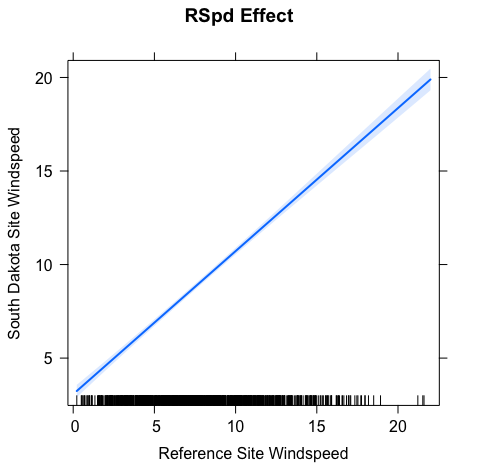
\includegraphics[width=\textwidth]{Rplot01.png}
      \end{subfigure}
      \hfill
      \begin{subfigure}[b]{0.45\textwidth}
          \centering
          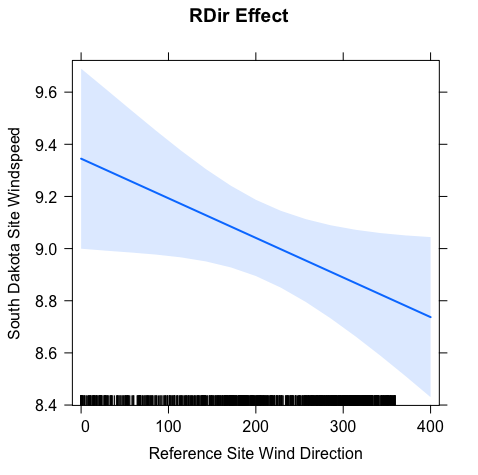
\includegraphics[width=\textwidth]{Rplot1.png}
      \end{subfigure}
  \end{figure}




















      \end{enumerate}
      
    \end{exercise}


\end{exercise}

\end{document}





















